\documentclass{beamer}
\usetheme{afm}

\title{Bootstrap Technique}
\author{Matteo Sani \href{mailto:matteo.sani@unisi.it}{matteo.sani@unisi.it}}

\begin{document}
\begin{frame}[plain]
  \maketitle
\end{frame}

\begin{frame}{Overnight Index Swap}
\begin{itemize}
\item Interest rate swaps (IRS) are usually used to mitigate the risks of fluctuations of interest rates, or to benefit from lower rates. 
\item An Overnight Index Swap (OIS) is a particular kind of IRS which pays a floating coupon, determined a pre-determined index of a daily overnight reference rate (e.g €STR), against a fixed coupon.  
\item An OIS is defined by:
\begin{itemize}
  \item a notional amount $N$;
  \item a starting date $d_0$;
  \item a sequence of payment dates $d_1,...,d_n$;
  \item a fixed rate $K$.
\end{itemize}
\item For simplicity in the following we assume the fixed and floating legs to have the same notional and payment dates, although this is not necessarily always the case in practice.
\end{itemize}
\end{frame}

\begin{frame}{OIS Valuation}
\begin{itemize}
\item To compute the NPV of such products it is necessary to sum the discounted values of each leg cash flows (full derivation in the notes)
\begin{tabular}{|c|c|}
\hline
 Floating Leg & Fixed Leg \\
\hline
$\mathrm{NPV}_{\mathrm{float}} = N \cdot [D_{\mathrm{OIS}}(d_0) - D_{\mathrm{OIS}}(d_n)]$ & $\mathrm{NPV}_{\mathrm{fixed}} = N\cdot K\cdot \sum_{i=1}^{n}D_{\mathrm{OIS}}(d_{i})\frac{d_i - d_{i-1}}{360}$ \\
\hline
\end{tabular}
\\\vspace{0.05cm}
where $D_{\mathrm{OIS}}(d)$ is the discount factors implied by OIS prices (\textbf{we will see how to derive it}).
\item We will always look at these products from the point of view of the \emph{receiver of the floating leg}
\begin{equation}
\mathrm{NPV}_{\mathrm{OIS}} = \mathrm{NPV}_{\mathrm{float}} - \mathrm{NPV}_{\mathrm{fixed}}
\end{equation}
\item The $\frac{1}{360}$ fraction appears because €STR rates are quoted using the ACT/360 day-count convention:
\begin{itemize} 
  \item other currencies might have different conventions;  
  \item in addition we are making the simplifying assumption of ignoring weekends and holidays: each overnight rate is valid for only one day.
  \end{itemize}
\end{itemize}
\end{frame}

%\begin{frame}{OvernightIndexSwap Class}
%\begin{itemize}
%\item Let's write a class to represent OIS and compute its value given a specific discount curve
%\begin{itemize}
%    \item attributes: start_date, nominal, fixed leg rate and payment dates;
%    \item methods: two to compute NPVs of floating and fixed legs respectively and one to compute the swap value. 
%    \end{itemize}
% \item In order to avoid future bugs and to provide users with the correct information to use a class it is always a good practice to document your code.
% \item Documentation can be written inline beside the class code using multiline strings ($\texttt{"""}$) below each method to describe the purpose and the needed parameters.
% 
%# define OIS class
%from finmarkets import generate_dates
%
%class OvernightIndexSwap:
%  """
%  Class to manage Overnight Index Swap contracts
%  Parameters:
%  nominal: the nominal of the contract
%  start_date: the initial date of the contract
%  maturity_months: the maturity to be expressed in months 
%  fixed_rate: rate of the "fixed leg"
%  """
%  def __init__(self, nominal, start_date, maturity_months, fixed_rate):
%      self.start_date = start_date
%      self.nominal = nominal
%      self.fixed_rate = fixed_rate
%      self.payment_dates = generate_dates(start_date, maturity_months)
%      
%  def npv_floating(self, dc):
%    """
%    Method to compute the floating leg NPV
%    Parameters:
%    dc: dicscount curve to be used in the calculation
%    """
%    return self.nominal * (dc.df(self.payment_dates[0]) - dc.df(self.payment_dates[-1]))
%  
%  def npv_fixed(self, dc):
%    """
%    Method to compute the fixed leg NPV
%    Parameters:
%    dc: dicscount curve to be used in the calculation
%    """
%    val = 0
%    for i in range(1, len(self.payment_dates)):
%        val += dc.df(self.payment_dates[i]) * \
%                (self.payment_dates[i] - self.payment_dates[i-1]).days/360 
%    return self.nominal*self.fixed_rate*val
%  
%  def npv(self, dc):
%    """
%    Method to compute the contract NPV seen from the point of view of the 
%    receiver of the floating leg.
%    Parameters:
%    dc: dicscount curve to be used in the calculation
%    """
%    return self.npv_floating(dc) - self.npv_fixed(dc)
%        
% #### Example
% 
% * Let's test the class with this [discount curve](https://github.com/matteosan1/finance_course/raw/develop/libro/input_files/discount_factors_2022-10-05.xlsx).
% 
%# test the class
%import pandas as pd
%from datetime import date
%from finmarkets import DiscountCurve
%from dateutil.relativedelta import relativedelta
%
%start_date = date(2020, 10, 21)
%ois = OvernightIndexSwap(1e6,
%                         start_date, 
%                         36,
%                         0.025)
%
%df = pd.read_excel("https://github.com/matteosan1/finance_course/raw/develop/libro/input_files/discount_factors_2022-10-05.xlsx")
%pillars = [start_date + relativedelta(months=i) for i in df['months']]
%dfs = df['dfs']
%
%curve = DiscountCurve(pillars, dfs)
%
%print ("OIS NPV: {:.2f}".format(ois.npv(curve)))
%
%OIS NPV: -2096.44

\begin{frame}{Discount Factor Determination (Bootstrap)}
\begin{itemize}
\item Our ultimate goal is to take a series of Overnight Index Swap quotations, and determine the discount factors implied by their prices. 
\item The employed technique is called \emph{bootstrap}: this is the ABC of financial mathematics, since you always need a discount curve to price a contract.
\item We concentrate on €STR swaps in order to build an EUR discount curve.
\item The assumption underlying bootstrap is that market quotes represent the \emph{fair} prices of the OIS:
\begin{itemize}
  \item by fair price we mean an estimate of what a willing buyer would pay a willing seller for a given asset, assuming both have a reasonable knowledge of the asset's worthiness;
  \item by definition market quotes make the swap NPVs null.
  \end{itemize}
  \end{itemize}
\end{frame}  
  
\begin{frame}{The Algorithm}
\begin{itemize} 
\item In finance, \emph{bootstrap} is a method for constructing a yield curve from the prices of a set of coupon-bearing products (e.g. bonds and swaps) using only few selected products, it is possible to derive rates for all possible maturities.
\item The term structure of spot rates is obtained from the yields by \emph{forward substitution}, in other words by solving for them recursively. 
\end{itemize}
\end{frame} 

\begin{frame}[fragile]{Example}
\begin{itemize}
\item Consider five bonds (yearly fixed coupon of 4\%, 5\%, 6\%, 7\% and 8\% respectively) with maturities ranging from 1 to 5 years, each having a value of €100 and \emph{traded at par} (traded at its face value). 
\item To determine the yield curve proceed as follows:
\begin{enumerate}
   \item at the end of first year the discounted cash flow of the first bond is €104 (principal + coupon) times the discount factor, so the implied 1 year rate can be found by solving
   \begin{equation*}
 100 = \cfrac{104}{(1 + r_{1y})}\implies r_{1y} =  104/100 - 1 = 4\%
 \end{equation*}
 \item at the end of second year the sum of the cash flows of the second bond can be compared to its trading price to compute the 2-year spot rate $r_{2y}$ (using the previously derived value of $r_{1y}$)
    \begin{equation*}
    \begin{gathered}
 100 = \cfrac{5}{(1 + r_{1y})} + \cfrac{105}{(1 + r_{2y})^{2}} \\
 100 = 5 / (1 + 0.04) + 105 / (1 + r_{2y})^{2}\qquad\Rightarrow\qquad r_{2y}^2  + 2 r_{2y}  - 0.103030 = 0
 \end{gathered}
 \end{equation*}
 \end{enumerate}
 \end{itemize}
\end{frame}
 
\begin{frame}[fragile]{Example}
\begin{itemize}
 This second order equation can be solved either by hand or with \texttt{numpy.roots}.
 \begin{equation*}
    r_{2y} = - 1 \pm \sqrt{1 + 0.103030} = \begin{cases}-2.05023 \\ 0.0502\end{cases}
    \end{equation*}
    
 \begin{ipython}
import numpy as np
np.roots([1, 2, -0.103030])
 \end{ipython}
 \begin{ioutput}
 array([-2.05025235,  0.05025235])
\end{ioutput}
\item From the third year on we get equation of third order (or more) which are not easily analitically solvable (fifth year):
 \begin{equation*}
 100 = \cfrac{8} {(1 + r_{1y})} + \cfrac{8} {(1 + r_{2y})^{2}}+ \cfrac{8} {(1 + r_{3y})^{3}} + \cfrac{8} {(1 + r_{4y})^{4}} + \cfrac{108} {(1 + r_{5y})^{5}}
 \end{equation*}
\end{itemize}
\end{frame}  
 
 \begin{frame}[fragile]{Example}
 \begin{itemize}
 \item Assuming we have already determined the previous rates:
 \begin{center}
 \begin{tabular}{|c|c|c|c|}
 \hline
  years & coupon rate & bond price & rate \\
 \hline
 1 & 1\% & 100 & 4.00\% \\
 \hline
 2 & 2\% & 100 & 5.02\% \\
 \hline
 3 & 3\% & 100 & 6.08\% \\
 \hline
 4 & 4\% & 100 & 7.19\% \\
 \hline
 5 & 5\% & 100 & ???? \\
 \hline
 \end{tabular}
 \end{center}
 \item Solving the previous equation means to find its zeros: the values of $\hat{x}$ for which $f(\hat{x})=0$.
 \item There are various methods to solve this problem (which is also called root-finding), the simplest being the \emph{bisection method}.
% ![](https://drive.google.com/uc?id=1Zt18h9fRo65Er5V9iJBdOpX4trcytLSW)
 \end{itemize}
 \end{frame} 
 
\begin{frame}[fragile]{Example}
\begin{itemize}
 \item In \emph{python} this algorithm is implemented in \texttt{scipy.optimize.bisect}.
 
\begin{ipython}
import numpy as np
from scipy.optimize import bisect
 
def f(y):
    return 8/(1+0.04) + 8/np.power((1+0.0502), 2) + 8/np.power((1+0.0608), 3) + 
    8/np.power((1+0.0719), 4) + 108/np.power((1+y), 5) - 100
 
print (f"{bisect(f, 0, 1):.4f}")
\end{ipython}
\begin{ioutput} 
 0.08359
\end{ioutput} 
\item An interesting alternative is the \emph{Brent method} (\texttt{scipy.optimize.brentq}).

\begin{ipython}
from scipy.optimize import brentq
 
print (f"{brentq(f, 0, 1):.4f}")
\end{ipython}
\begin{ioutput} 
 0.08359
\end{ioutput} 
 \end{itemize}
 \end{frame} 
 
\begin{frame}[fragile]{Example}
\begin{itemize}
\item The very same mechanism can be generalized to more maturities to get a more detailed yield curve: 
 
\begin{equation*}
 \begin{cases}
 f_1(r_1, p_1) = 0 \\
 f_2(r_1, r_2, p_2) = 0 \\
 f_3(r_1, r_2, r_3, p_3) = 0 \\
 f_4(r_1, r_2, r_3, r_4, p_4) = 0 \\
 \cdots
 \end{cases}
 \end{equation*}
where $r_i$ are the unknown spot rates and $p_i$ the market quotes of the considered products. 
 
 \item The iterative procedure we have applied before exploits the first equation to find $r_1 = f_1^{-1}(p_1)$, the second to find $r_2 = f_2^{-1}(r_1, p_2)$ and so on...
\end{itemize}
\end{frame} 
 
\begin{frame}{Minimization Algorithm}
    \begin{itemize}
 	\item Find the dimensions that will minimize the costs to manufacture a cylindrical can of volume $330~\mathrm{cm}^3\;(33~\mathrm{cl})$:
   	 cheaper can $\rightarrow$ less aluminium $\rightarrow$ smaller surface given the volume.
   	 \begin{columns}
   	 	\column{0.5\linewidth}
 	\begin{figure}[htb]
 		\begin{center}
 			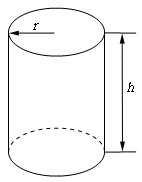
\includegraphics[width=0.40\linewidth]{cylinder}
 		\end{center}
 	\end{figure}
 \column{0.5\linewidth}
 	\begin{equation*}
 	S(r, h) = 2\pi rh + 2\cdot(\pi r^2)
 \end{equation*}
 	\item The volume is fixed to $330~\mathrm{cm}^3$ so we can remove $h$ from the previous equation:
 	\begin{equation*}
 	V = \pi r^2 h = 330\quad\implies h = \cfrac{330}{\pi r^2}
 	\end{equation*}
 \end{columns}
	\item The surface function to be minimized is:
	\begin{equation*}
	S(r) = 2\pi rh + 2\cdot(\pi r^2) = \cfrac{2\cdot 330}{r} + 2\cdot(\pi r^2) 
\end{equation*}
\end{itemize}
\end{frame}

\begin{frame}{Minimization Algorithm}
 \begin{enumerate}
  \item define an \emph{objective function} i.e. the function that is actually minimized to reach our goal (in this example the can area function);
  \item  set the initial value of the unknown parameters and their range of variability; we are going to start with $r=1~\mathrm{cm}$ and let it varies between $1~\textrm{mm}$ and $1~\textrm{m}$;
  \item finally run the algorithm (\texttt{scipy.optimize.minimize}):
  \begin{itemize}
     \item compute the objective function value;
     \item move the parameter values ($r$ in our example) to find a smaller value of the objective function (e.g. following the derivative direction w.r.t. each parameter); in case constraints are defined, they will be considered when the parameter values are varied;
     \item repeat until further variations of the values won’t change significantly the objective function (i.e. we have found a minimum of the function so the minimization process is completed !).
    \end{itemize}
\end{enumerate}
\end{frame}

\begin{frame}{Back to OIS Bootstrap}
\begin{itemize} 
 \item In the latter formulation we gave bootstrap requires to minimize simultaneously the NPV's of a set of OIS;
 
 \begin{equation}
 \mathrm{Objective Function} =	f_1^2(\hat{r}_1,p_1) + f_2^2(\hat{r}_1, \hat{r}_2,p_2) + \ldots =\sum_{i=1}^{n}\mathrm{NPV}^\mathrm{OIS}_i(\mathcal{C})^2
 \end{equation}
 
 \item  The only unknown parameter of each NPV is the discount curve $\mathcal{C}$ (i.e. \textbf{the algorithm will adjust the unknown discount factors of $\mathcal{C}$ to reach the minimum}).
 \item In the previous example there was a single parameter involved in the minimization i.e. the can radius.
\end{itemize}
\end{frame}

\begin{frame}{Back to OIS Bootstrap}
	\begin{itemize} 
 \item A discount curve is characterized by pillar dates ($\mathbf{d}$) and discount factors ($\mathbf{x}$):
we haven't yet identified a constraint on how many points the curve needs to be made of (\emph{too many or too few points may prevent us from finding the solution}).
  \item \textbf{It makes sense to choose the number of parameters (degrees of freedom) to match the number of market quotes} (set the pillar dates equal to the set of the swap expiry dates).
 
 \begin{equation}
  \mathrm{min}_{\mathbf{x}} \left\{\sum_{i=1}^{N}\mathrm{NPV}^\mathrm{OIS}_i( \mathcal{C}(\mathbf{x}))^2\right\}
 \end{equation}
\end{itemize}
\end{frame} 
     
\end{document}
